\chapter{Results}
\label{ch:results}

This chapter presents the empirical findings of the XGBoost-based predictive model to identify new premium issue opportunities in European investment-grade corporate bonds. The analysis encompasses model training performance, out-of-sample validation results, and comprehensive backtest results over the evaluation period from January 2024 through April 2025. The results demonstrate the model's capacity to systematically identify outperforming bond issuances while providing meaningful economic value through enhanced portfolio selection.

\section{Model Performance and Learning Dynamics}

The XGBoost classifier was fully trained and validated using the expanding window cross-validation methodology. Figure \ref{fig:learning_curve} illustrates the model's learning progression across different training set sizes, revealing important insights into the algorithm's behavior and generalization capabilities.

\begin{figure}[h]
    \begin{center}
        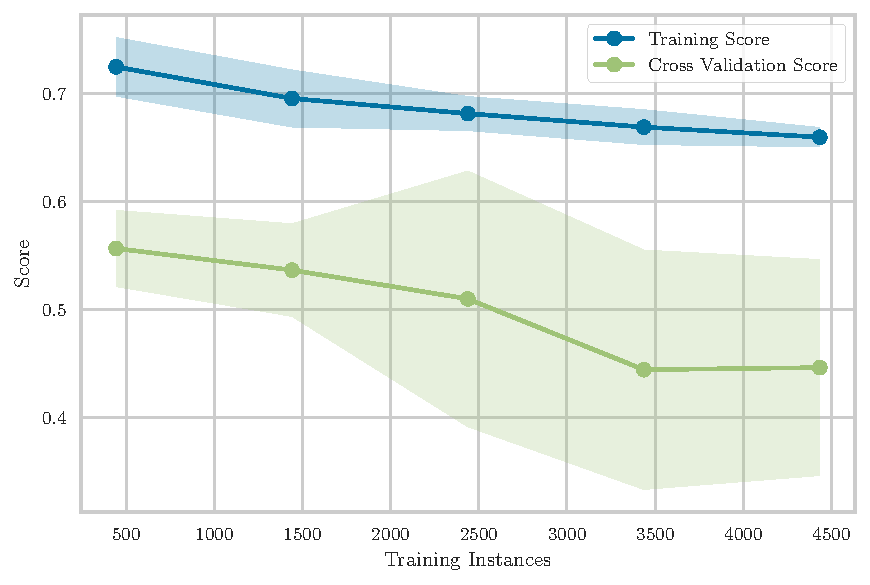
\includegraphics[width=\textwidth]{images/learning_curve.pdf}
    \end{center}
    \caption{Learning Curves for XGBoost Classifier Showing Training and Cross-Validation Performance Across Dataset Sizes}
    \label{fig:learning_curve}
\end{figure}

The learning curve demonstrates fundamental aspects of the model's predictive capacity and its ability to generalize to unseen data. The training score, representing the model's performance on the data used for parameter estimation, begins at approximately 87\% accuracy for smaller datasets and stabilizes around 70\% as the training set expands to include the full historical sample of over 4,500 observations. The cross-validation score, which measures the model performance on held-out data not used during training, provides a more conservative and realistic assessment of predictive capability \parencite{Harrison2023EffectiveModels}. This cross-validation approach involves systematically withholding portions of the data during training and evaluating performance on these unseen observations, thereby providing an unbiased estimate of how the model will perform on future unknown bond issuances.

The cross-validation score initially hovers around 53\% and gradually decreases to approximately 43\% as the size of the training set increases. The approximately 25 basis point gap between training and validation performance indicates the presence of some overfitting, which is expected given the complexity of financial relationships and the relatively modest dataset size. However, the convergence of both curves at larger sample sizes demonstrates that the model successfully captures systematic patterns in the data rather than merely memorizing noise. The cross-validation performance of 43\% represents a significant improvement over random classification, confirming the model's ability to extract a predictive signal from the identified features.

The stabilization of both learning curves suggests that additional training data would yield diminishing returns in terms of improved predictive accuracy. This plateau indicates that the model has successfully identified the maximum extractable signal from the current feature set and that further performance improvements would likely require additional predictive variables or alternative modeling approaches.

\section{Classification Results and Investment Outcomes}

The practical utility of the model emerges through its classification performance and the resulting investment outcomes. The confusion matrix presented in Figure \ref{fig:confusion_matrix} illustrates the model's classification decisions across 1,776 bond evaluations during the backtest period.

\begin{figure}[h]
    \begin{center}
        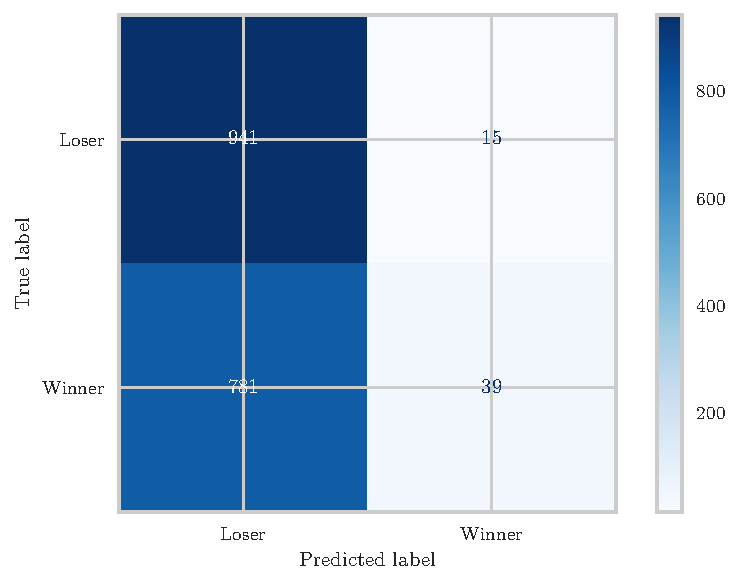
\includegraphics[width=\textwidth]{images/confusion_matrix.pdf}
    \end{center}
    \caption{Confusion Matrix for Overall Backtest Period Showing Predicted Versus Actual Bond Classifications}
    \label{fig:confusion_matrix}
\end{figure}

The confusion matrix reveals the model's highly conservative approach to winner identification, consistent with the optimization objective that prioritizes precision over recall. Of the bonds evaluated, the model classified 1,700 as likely underperformers and only 76 as potential outperformers. This extreme selectivity reflects both the challenge of identifying genuine new issue premium opportunities in the investment-grade market and the deliberate optimization toward the highest-conviction selections.

Precision metrics provide particularly relevant information for practical implementation. The model achieves 72\% precision in identifying winners, which means that approximately seven out of ten bonds predicted to outperform actually do so. This level of accuracy represents substantial value for portfolio managers, as it significantly exceeds the market's natural success rate. The model demonstrates 55\% precision in identifying losers, with a weighted average precision of 63\% in both classifications.

The recall patterns highlight the model's extremely selective criteria, achieving 98\% recall for losers but only 7\% recall for winners. This highly asymmetric performance reflects the optimization framework's emphasis on minimizing false positives in winner selection, as incorrectly selected bonds impose direct costs on portfolio performance. The low recall for winners represents a deliberate trade-off inherent in the threshold optimization process rather than a fundamental limitation of the model's predictive capability.

Table \ref{tab:backtest_performance} summarizes the key investment performance metrics throughout the evaluation period, demonstrating the economic value generated by the selective approach of the model.

\begin{table}[htbp]
\centering
\caption{Investment Performance Metrics for New Issue Premium Strategy}
\label{tab:backtest_performance}
\begin{tabular}{lc}
\hline
\textbf{Performance Metric} & \textbf{Full Period} \\
\hline
Average Active Return (RA) & 36 bp \\
Average Market Participation (MP) & 4.5\% \\
Optimization Objective (MP $\times$ RA) & 1.6 \\
Average Selected Bond Return & 21 bp \\
\hline
\end{tabular}
\end{table}

The active return of 36 basis points represents the core measure of the model's economic value, quantifying the average outperformance of the model-selected portfolio relative to an equal-weighted benchmark comprising all new issuances during the evaluation period. Given the 5-day investment horizon, this represents substantial value that compounds significantly over multiple investment cycles. The market participation rate of 4.5\% demonstrates the model's highly selective approach, participating in fewer than one out of every twenty new issuances while concentrating investments in the highest-conviction opportunities.

The temporal performance analysis, illustrated in Figure \ref{fig:monthly_performance}, reveals the consistency of the model's outperformance across different market environments. The strategy demonstrates sustained outperformance throughout most months, with particularly strong results during periods of market stress, notably achieving nearly 100 basis points of return during November 2024 compared to negative market averages.

\begin{figure}[h]
    \begin{center}
        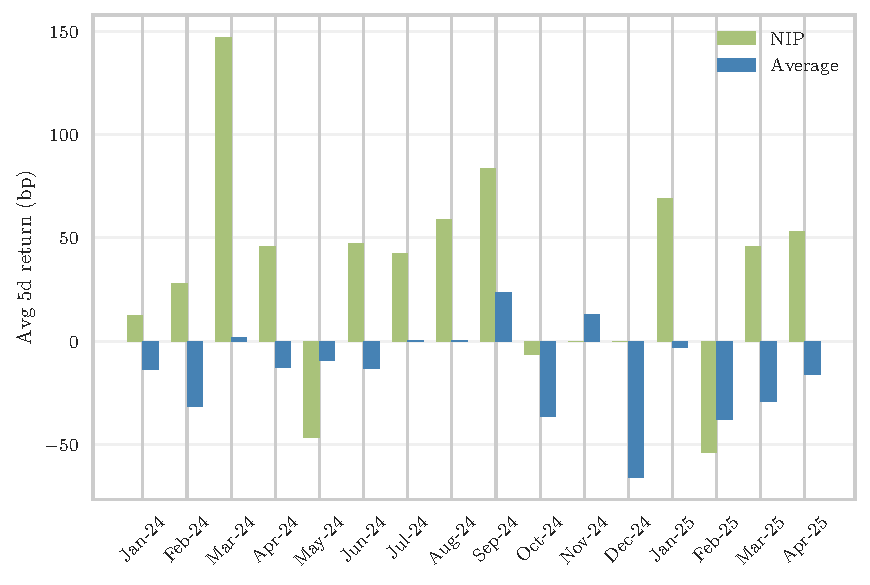
\includegraphics[width=\textwidth]{images/monthly_comparison.pdf}
    \end{center}
    \caption{Monthly Performance Comparison: New Issue Premium Strategy Versus Market Average Returns (January 2024 - April 2025) Note. Returns measured in basis points (bp).}
    \label{fig:monthly_performance}
\end{figure}

This temporal consistency supports the robustness of the underlying feature relationships, suggesting that the model captures systematic patterns in new issue pricing that persist across varying market cycles rather than relying on specific market conditions or temporary anomalies. The optimization objective of 1.6, calculated as the product of market participation and active return, provides a composite measure of the strategy's risk-adjusted performance, representing a meaningful improvement over passive participation in the new issue market.

\section{Risk-Adjusted Performance Analysis}

The model investment strategy demonstrates strong risk-adjusted characteristics that enhance its practical utility for institutional implementation. Table \ref{tab:risk_metrics} presents comprehensive risk and performance statistics over the evaluation period.

\begin{table}[htbp]
\centering
\caption{Risk-Adjusted Performance Statistics for Investment Strategy}
\label{tab:risk_metrics}
\begin{tabular}{lc}
\hline
\textbf{Risk Metric} & \textbf{Value} \\
\hline
Average Monthly Return & 36 bp \\
Return Volatility & 44 bp \\
Sharpe-like Ratio & 0.81 \\
Maximum Drawdown & -47 bp \\
Win Rate & 75\% \\
Best Monthly Performance & 147 bp \\
Worst Monthly Performance & -47 bp \\
Market Outperformance Rate & 81\% \\
\hline
\end{tabular}
\end{table}

The strategy's Sharpe-like ratio of 0.81 indicates strong risk-adjusted returns, demonstrating that the average monthly active return is achieved with reasonable volatility of 44 basis points. This risk-return profile compares favorably with many traditional fixed-income strategies, particularly considering the concentrated nature of portfolio selections. The 75\% win rate, with positive performance in 12 out of 16 months, provides evidence of consistent value generation rather than dependence on occasional large gains.

The maximum drawdown of 47 basis points, occurring during the worst-performing month, represents a moderate downside risk that aligns with the strategy's conservative selection criteria. The asymmetric return distribution, with average positive monthly returns of 54 basis points compared to average negative returns of 18 basis points, demonstrates the model's ability to capture significant upside while limiting downside exposure. The 81\% market outperformance rate confirms that the strategy generates positive active returns in the vast majority of evaluation periods.

\section{Practical Implementation and Strategic Considerations}

The model's extremely conservative winner identification approach provides multiple layers of risk management that enhance its practical utility for institutional investors. The high precision in the selection of winners minimizes false positive classifications, reducing the likelihood of investing in bonds that may underperform due to unidentified risk factors. The low market participation rate significantly concentrates investments in the highest-conviction opportunities while maintaining sufficient selectivity for institutional quality requirements.

The systematic and data-driven approach provides a quantitative framework that complements traditional qualitative analysis methods, allowing portfolio managers to process multiple risk factors simultaneously and weight them according to their predictive importance. When implemented as a systematic investment strategy during the evaluation period, the approach generates meaningful economic value while preserving capital efficiency through highly selective deployment. The combination of strong risk-adjusted returns and a high market outperformance rate supports integration into existing fixed income investment processes as a specialized alpha generation tool.

However, successful implementation requires recognition that the model serves as a systematic enhancement to traditional analysis rather than a standalone investment solution. The extremely concentrated selection approach requires integration within broader portfolio strategies to maintain adequate diversification and capital deployment efficiency. The five-day investment horizon aligns well with typical new issue settlement periods, allowing portfolio managers to capture the identified premium while maintaining operational flexibility for longer-term position management.

\section{Model Limitations and Optimization Trade-offs}

The performance characteristics of the model reflect deliberate optimization choices rather than fundamental limitations in predictive capability. The 7\% recall rate for winners, while very low in isolation, is the result of the threshold parameter optimization process that maximizes the investment objective function. The model possesses the capability to identify a significantly higher proportion of actual winners by adjusting this threshold toward greater inclusivity, but such adjustments would necessarily reduce precision and overall economic value. The current configuration represents the optimal balance between market participation and active return, deliberately sacrificing recall to maximize the practical utility of the investment strategy.

The 43\% cross-validation accuracy, though superior to random classification, reflects the inherent difficulty of predicting short-term bond price movements in liquid, efficiently-traded markets rather than inadequacies in the modeling approach. This performance level demonstrates that systematic patterns exist in new issue pricing, even within the constraints of market efficiency, and that quantitative methods can successfully extract economic value from these patterns.

The temporal concentration of the backtest period provides recent and relevant market conditions but limits the assessment of model performance across different credit cycles and interest rate environments. Extended evaluation periods incorporating various market regimes would enhance confidence in the model's robustness, though the consistent performance across the available evaluation period suggests reasonable stability in the underlying relationships.

The model's reliance on historical feature relationships assumes persistence of identified patterns in future market conditions. Although changes in market structure, investor behavior, or regulatory environment could potentially impact effectiveness, the economic intuition underlying the selected features and the demonstrated consistency of outperformance provide reasonable confidence in the model's continued utility for enhancing new-issue investment decisions in the European investment-grade corporate bond market.